\documentclass[UTF8]{ctexart}

\usepackage{amsmath,amssymb}
\usepackage[a4paper,margin=18mm]{geometry}
\usepackage{xcolor}
\usepackage{tikz}
\usepackage{pgfplots}
\pgfplotsset{compat=1.18}

\setlength{\parindent}{2em}
\setlength{\parskip}{0.4em}

\usepackage{tikz}
\usetikzlibrary{calc,arrows,angles,quotes,intersections}

\begin{document}
	
	
\section{第 6 讲：圆锥曲线核心知识体系（完整还原版）}

\noindent\textbf{整理说明：}本文按《王老师教案.pdf》第 59--79 页的授课顺序整理。
原稿以课堂手绘图和口头推导为主；下文保留原有结论，并补足每条结论成立的曲线、
焦点、支别与角度条件。为避免歧义，椭圆、双曲线均默认焦点在 $x$ 轴上，
抛物线默认方程为 $y^2=2px\ (p>0)$。
	
	\subsection{圆锥曲线的统一定义}
	
	圆锥曲线可以统一理解为：
	平面内动点 $P$ 到定点 $F$ 的距离与到定直线 $l$ 的距离之比为常数 $e$，即
	\[
	\frac{PF}{d(P,l)}=e.
	\]
	其中 $e$ 称为离心率。
	
	\[
	\begin{cases}
		0<e<1, & \text{椭圆},\\
		e=1, & \text{抛物线},\\
		e>1, & \text{双曲线}.
	\end{cases}
	\]
	
	\begin{center}
		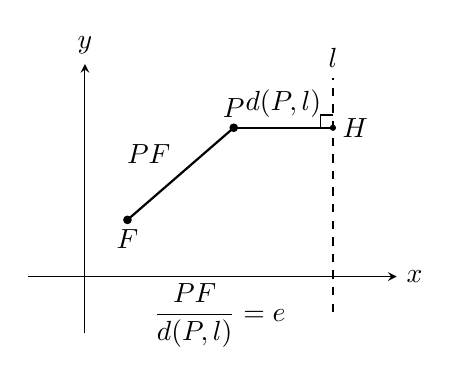
\begin{tikzpicture}[scale=0.9,>=stealth]
			\draw[->] (-0.8,0)--(4.4,0) node[right]{$x$};
			\draw[->] (0,-0.8)--(0,3.0) node[above]{$y$};
			
			\coordinate (F) at (0.6,0.8);
			\coordinate (P) at (2.1,2.1);
			\coordinate (H) at (3.5,2.1);
			
			\draw[dashed,thick] (3.5,-0.5)--(3.5,2.8) node[above]{$l$};
			\draw[thick] (F)--(P) node[midway,above left]{$PF$};
			\draw[thick] (P)--(H) node[midway,above]{$d(P,l)$};
			\draw[fill] (F) circle (1.5pt) node[below]{$F$};
			\draw[fill] (P) circle (1.5pt) node[above]{$P$};
			\draw[fill] (H) circle (1pt) node[right]{$H$};
			
			\draw ($(H)+(0,0.18)$)--($(H)+(-0.18,0.18)$)--($(H)+(-0.18,0)$);
			
			\node at (1.9,-0.55) {$\displaystyle \frac{PF}{d(P,l)}=e$};
		\end{tikzpicture}
	\end{center}
	
	
	\subsection{圆锥截线与离心率}
	
	设圆锥母线与轴的夹角为 $\alpha$，截面与圆锥轴的夹角为 $\beta$，则有
	\[
	e=\frac{\cos\beta}{\cos\alpha}.
	\]
	
	因此：
	\[
	\begin{cases}
		\beta>\alpha, & e<1,\quad \text{椭圆},\\
		\beta=\alpha, & e=1,\quad \text{抛物线},\\
		\beta<\alpha, & e>1,\quad \text{双曲线}.
	\end{cases}
	\]
	
	\begin{center}
		\begin{tikzpicture}[scale=0.75,>=stealth]
			
			% 椭圆截线
			\begin{scope}[xshift=0cm]
				\draw[thick] (0,2.2)--(-1.5,-1.2);
				\draw[thick] (0,2.2)--(1.5,-1.2);
				\draw[dashed] (0,2.2)--(0,-1.2);
				\draw (0,-1.2) ellipse (1.5 and 0.28);
				\draw[red,thick] (-1.0,0.25)--(1.05,0.65);
				\node at (0,-1.85) {$\beta>\alpha$};
				\node at (0,-2.35) {$e<1,\ \text{椭圆}$};
			\end{scope}
			
			% 抛物线截线
			\begin{scope}[xshift=4.6cm]
				\draw[thick] (0,2.2)--(-1.5,-1.2);
				\draw[thick] (0,2.2)--(1.5,-1.2);
				\draw[dashed] (0,2.2)--(0,-1.2);
				\draw (0,-1.2) ellipse (1.5 and 0.28);
				\draw[red,thick] (-1.3,-0.7)--(0.25,2.0);
				\node at (0,-1.85) {$\beta=\alpha$};
				\node at (0,-2.35) {$e=1,\ \text{抛物线}$};
			\end{scope}
			
			% 双曲线截线
			\begin{scope}[xshift=9.2cm]
				\draw[thick] (0,2.2)--(-1.5,-1.2);
				\draw[thick] (0,2.2)--(1.5,-1.2);
				\draw[dashed] (0,2.2)--(0,-1.2);
				\draw (0,-1.2) ellipse (1.5 and 0.28);
				\draw[red,thick] (-1.35,1.3)--(1.35,-0.3);
				\node at (0,-1.85) {$\beta<\alpha$};
				\node at (0,-2.35) {$e>1,\ \text{双曲线}$};
			\end{scope}
			
		\end{tikzpicture}
	\end{center}
	
	
	\subsection{椭圆的第一定义}
	
	椭圆是平面内到两个定点 $F_1,F_2$ 的距离之和为常数 $2a$ 的点的轨迹：
	\[
	PF_1+PF_2=2a.
	\]
	其中
	\[
	F_1F_2=2c,\qquad c^2=a^2-b^2,\qquad e=\frac{c}{a}.
	\]
	
	标准方程为
	\[
	\frac{x^2}{a^2}+\frac{y^2}{b^2}=1,\qquad a>b>0.
	\]
	
	\begin{center}
		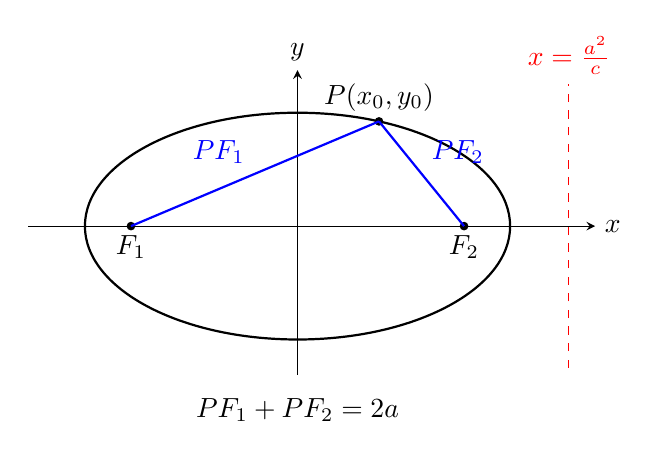
\begin{tikzpicture}[scale=0.9,>=stealth]
			\def\a{3}
			\def\b{1.6}
			\def\c{2.35}
			\pgfmathsetmacro{\px}{1.15}
			\pgfmathsetmacro{\py}{\b*sqrt(1-\px*\px/(\a*\a))}
			\pgfmathsetmacro{\dir}{\a*\a/\c}
			
			\draw[->] (-3.8,0)--(4.2,0) node[right]{$x$};
			\draw[->] (0,-2.1)--(0,2.2) node[above]{$y$};
			
			\draw[thick] (0,0) ellipse (\a cm and \b cm);
			
			\coordinate (F1) at (-\c,0);
			\coordinate (F2) at (\c,0);
			\coordinate (P) at (\px,\py);
			
			\draw[fill] (F1) circle (1.5pt) node[below]{$F_1$};
			\draw[fill] (F2) circle (1.5pt) node[below]{$F_2$};
			\draw[fill] (P) circle (1.5pt) node[above]{$P(x_0,y_0)$};
			
			\draw[thick,blue] (P)--(F1) node[midway,above left]{$PF_1$};
			\draw[thick,blue] (P)--(F2) node[midway,above right]{$PF_2$};
			
			\draw[dashed,red] (\dir,-2.0)--(\dir,2.0) node[above]{$x=\frac{a^2}{c}$};
			
			\node at (0,-2.6) {$PF_1+PF_2=2a$};
		\end{tikzpicture}
	\end{center}
	
	
	\subsection{椭圆的焦半径公式}
	
	若 $P(x_0,y_0)$ 在椭圆
	\[
	\frac{x^2}{a^2}+\frac{y^2}{b^2}=1
	\]
	上，则有
	\[
	PF_1=a+ex_0,\qquad PF_2=a-ex_0.
	\]
	
	\begin{center}
		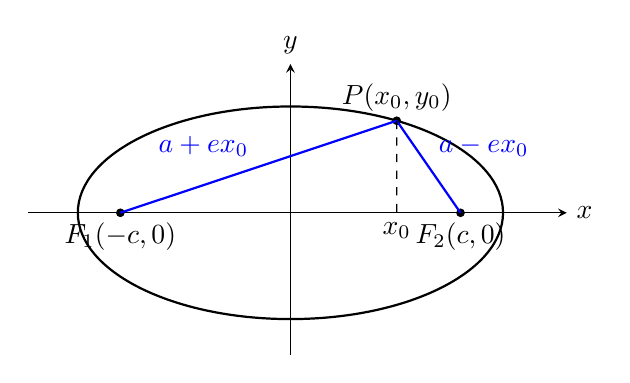
\begin{tikzpicture}[scale=0.9,>=stealth]
			\def\a{3}
			\def\b{1.5}
			\def\c{2.4}
			\pgfmathsetmacro{\px}{1.5}
			\pgfmathsetmacro{\py}{\b*sqrt(1-\px*\px/(\a*\a))}
			
			\draw[->] (-3.7,0)--(3.9,0) node[right]{$x$};
			\draw[->] (0,-2.0)--(0,2.1) node[above]{$y$};
			\draw[thick] (0,0) ellipse (\a cm and \b cm);
			
			\coordinate (F1) at (-\c,0);
			\coordinate (F2) at (\c,0);
			\coordinate (P) at (\px,\py);
			
			\draw[fill] (F1) circle (1.5pt) node[below]{$F_1(-c,0)$};
			\draw[fill] (F2) circle (1.5pt) node[below]{$F_2(c,0)$};
			\draw[fill] (P) circle (1.5pt) node[above]{$P(x_0,y_0)$};
			
			\draw[blue,thick] (F1)--(P) node[midway,above left]{$a+ex_0$};
			\draw[blue,thick] (F2)--(P) node[midway,above right]{$a-ex_0$};
			
			\draw[dashed] (P)--(\px,0) node[below]{$x_0$};
		\end{tikzpicture}
	\end{center}
	
	
	\subsection{椭圆的焦点三角形}
	
	设 $P$ 是椭圆上一点，连接 $PF_1,PF_2$ 得到焦点三角形
	\[
	\triangle PF_1F_2.
	\]
	若
	\[
	\angle F_1PF_2=\theta,
	\]
	则
	\[
	S_{\triangle PF_1F_2}=b^2\tan\frac{\theta}{2}.
	\]
	
	\begin{center}
		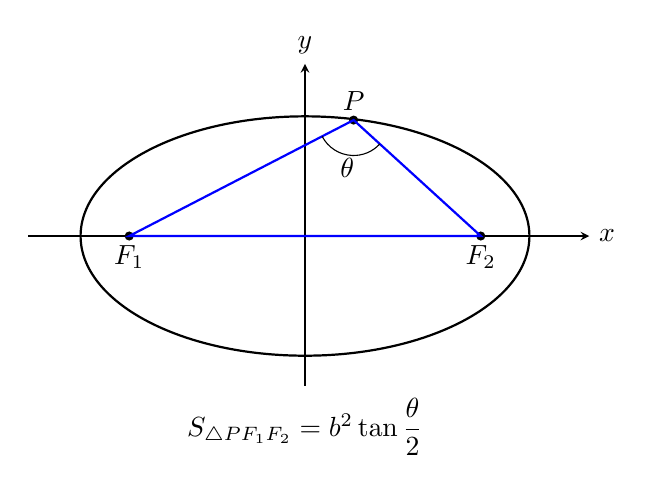
\begin{tikzpicture}[scale=0.95,>=stealth]
			\def\a{3}
			\def\b{1.6}
			\def\c{2.35}
			
			\coordinate (F1) at (-\c,0);
			\coordinate (F2) at (\c,0);
			\coordinate (P) at (0.65,1.55);
			
			\draw[->] (-3.7,0)--(3.8,0) node[right]{$x$};
			\draw[->] (0,-2.0)--(0,2.3) node[above]{$y$};
			\draw[thick] (0,0) ellipse (\a cm and \b cm);
			
			\draw[fill] (F1) circle (1.5pt) node[below]{$F_1$};
			\draw[fill] (F2) circle (1.5pt) node[below]{$F_2$};
			\draw[fill] (P) circle (1.5pt) node[above]{$P$};
			
			\draw[blue,thick] (P)--(F1)--(F2)--cycle;
			
			\pic [draw, "$\theta$", angle radius=0.45cm, angle eccentricity=1.35]
			{angle=F1--P--F2};
			
			\node at (0,-2.55) {$S_{\triangle PF_1F_2}=b^2\tan\dfrac{\theta}{2}$};
		\end{tikzpicture}
	\end{center}
	
	
	\subsection{椭圆的焦点弦}
	
	过焦点的弦称为焦点弦。设焦点弦 $AB$ 过焦点 $F$，且与长轴夹角为 $\theta$。
	令
	\[
	p=\frac{b^2}{a},
	\]
	则椭圆焦点弦长可以写成
	\[
	AB=\frac{2p}{1-e^2\cos^2\theta}.
	\]
	
	\begin{center}
		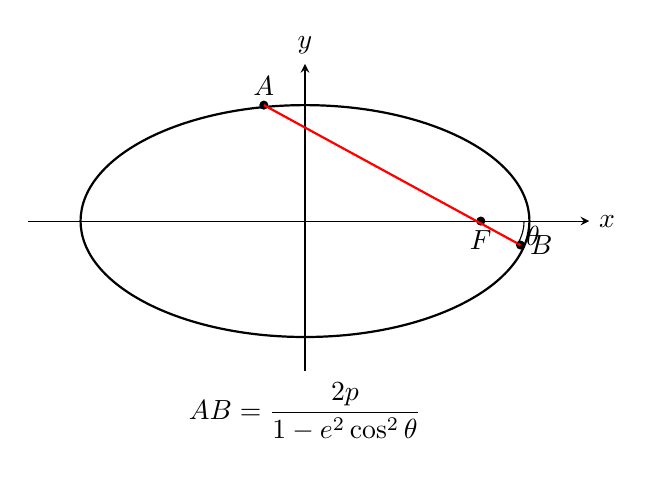
\begin{tikzpicture}[scale=0.95,>=stealth]
			\def\a{3}
			\def\b{1.55}
			\def\c{2.35}
			
			\draw[->] (-3.7,0)--(3.8,0) node[right]{$x$};
			\draw[->] (0,-2.0)--(0,2.1) node[above]{$y$};
			\draw[thick] (0,0) ellipse (\a cm and \b cm);
			
			\coordinate (F) at (\c,0);
			\coordinate (A) at (-0.55,1.55);
			\coordinate (B) at (2.88,-0.32);
			\coordinate (X) at (3.35,0);
			
			\draw[fill] (F) circle (1.5pt) node[below]{$F$};
			\draw[fill] (A) circle (1.5pt) node[above]{$A$};
			\draw[fill] (B) circle (1.5pt) node[right]{$B$};
			
			\draw[red,thick] (A)--(B);
			\draw[dashed] (F)--(X);
			
			\pic [draw, "$\theta$", angle radius=0.55cm, angle eccentricity=1.25]
			{angle=B--F--X};
			
			\node at (0,-2.55) {$AB=\dfrac{2p}{1-e^2\cos^2\theta}$};
		\end{tikzpicture}
	\end{center}
	
	
	\subsection{椭圆的切线与光学性质}
	
	椭圆
	\[
	\frac{x^2}{a^2}+\frac{y^2}{b^2}=1
	\]
	在点 $P(x_0,y_0)$ 处的切线方程为
	\[
	\frac{x_0x}{a^2}+\frac{y_0y}{b^2}=1.
	\]
	
	椭圆的光学性质是：从一个焦点发出的光线经椭圆反射后，会经过另一个焦点。
	
	\begin{center}
		\begin{tikzpicture}[scale=0.95,>=stealth]
			\def\a{3}
			\def\b{1.5}
			\def\c{2.35}
			
			\coordinate (F1) at (-\c,0);
			\coordinate (F2) at (\c,0);
			\coordinate (P) at (0.8,1.45);
			
			\draw[->] (-3.7,0)--(3.8,0) node[right]{$x$};
			\draw[->] (0,-2.0)--(0,2.1) node[above]{$y$};
			\draw[thick] (0,0) ellipse (\a cm and \b cm);
			
			\draw[fill] (F1) circle (1.5pt) node[below]{$F_1$};
			\draw[fill] (F2) circle (1.5pt) node[below]{$F_2$};
			\draw[fill] (P) circle (1.5pt) node[above]{$P$};
			
			\draw[blue,thick,->] (F1)--(P);
			\draw[blue,thick,->] (P)--(F2);
			
			% 切线近似画法
			\draw[red,thick] (-1.1,2.1)--(2.7,0.55) node[right]{切线};
			
			\node at (0,-2.55) {椭圆反射性质：$F_1\to P\to F_2$};
		\end{tikzpicture}
	\end{center}
	
	
	\subsection{双曲线的第一定义}
	
	双曲线是平面内到两个定点 $F_1,F_2$ 的距离之差的绝对值为常数 $2a$ 的点的轨迹：
	\[
	|PF_1-PF_2|=2a.
	\]
	标准方程为
	\[
	\frac{x^2}{a^2}-\frac{y^2}{b^2}=1,
	\]
	其中
	\[
	c^2=a^2+b^2,\qquad e=\frac{c}{a}>1.
	\]
	
	\begin{center}
		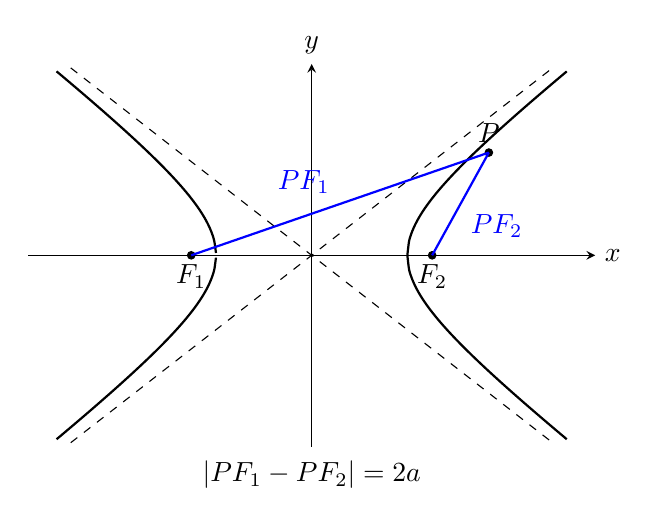
\begin{tikzpicture}[scale=0.9,>=stealth]
			\def\a{1.35}
			\def\b{1.05}
			\def\c{1.7}
			
			\draw[->] (-4,0)--(4,0) node[right]{$x$};
			\draw[->] (0,-2.7)--(0,2.7) node[above]{$y$};
			
			\draw[dashed] (-3.4,{-\b/\a*3.4})--(3.4,{\b/\a*3.4});
			\draw[dashed] (-3.4,{\b/\a*3.4})--(3.4,{-\b/\a*3.4});
			
			\draw[thick,domain=\a:3.6,samples=100,smooth]
			plot (\x,{\b*sqrt(\x*\x/(\a*\a)-1)});
			\draw[thick,domain=\a:3.6,samples=100,smooth]
			plot (\x,{-\b*sqrt(\x*\x/(\a*\a)-1)});
			\draw[thick,domain=-3.6:-\a,samples=100,smooth]
			plot (\x,{\b*sqrt(\x*\x/(\a*\a)-1)});
			\draw[thick,domain=-3.6:-\a,samples=100,smooth]
			plot (\x,{-\b*sqrt(\x*\x/(\a*\a)-1)});
			
			\coordinate (F1) at (-\c,0);
			\coordinate (F2) at (\c,0);
			\coordinate (P) at (2.5,1.45);
			
			\draw[fill] (F1) circle (1.5pt) node[below]{$F_1$};
			\draw[fill] (F2) circle (1.5pt) node[below]{$F_2$};
			\draw[fill] (P) circle (1.5pt) node[above]{$P$};
			
			\draw[blue,thick] (P)--(F1) node[midway,above left]{$PF_1$};
			\draw[blue,thick] (P)--(F2) node[midway,below right]{$PF_2$};
			
			\node at (0,-3.1) {$|PF_1-PF_2|=2a$};
		\end{tikzpicture}
	\end{center}
	
	
	\subsection{双曲线的焦点三角形}
	
	设 $P$ 是双曲线上一点，且
	\[
	\angle F_1PF_2=\theta.
	\]
	则焦点三角形面积公式为
	\[
	S_{\triangle PF_1F_2}=b^2\cot\frac{\theta}{2}.
	\]
	
	\begin{center}
		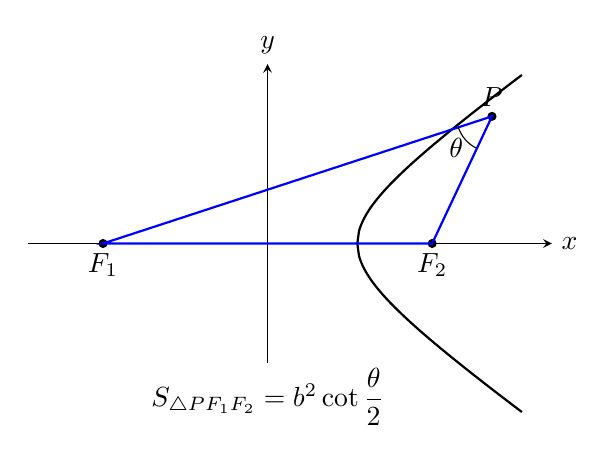
\begin{tikzpicture}[scale=0.95,>=stealth]
			\coordinate (F1) at (-2.2,0);
			\coordinate (F2) at (2.2,0);
			\coordinate (P) at (3.0,1.7);
			
			\draw[->] (-3.2,0)--(3.8,0) node[right]{$x$};
			\draw[->] (0,-1.6)--(0,2.4) node[above]{$y$};
			
			\draw[thick,domain=1.2:3.4,samples=100,smooth]
			plot (\x,{0.85*sqrt(\x*\x/1.44-1)});
			\draw[thick,domain=1.2:3.4,samples=100,smooth]
			plot (\x,{-0.85*sqrt(\x*\x/1.44-1)});
			
			\draw[fill] (F1) circle (1.5pt) node[below]{$F_1$};
			\draw[fill] (F2) circle (1.5pt) node[below]{$F_2$};
			\draw[fill] (P) circle (1.5pt) node[above]{$P$};
			
			\draw[blue,thick] (P)--(F1)--(F2)--cycle;
			
			\pic [draw, "$\theta$", angle radius=0.45cm, angle eccentricity=1.35]
			{angle=F1--P--F2};
			
			\node at (0,-2.05) {$S_{\triangle PF_1F_2}=b^2\cot\dfrac{\theta}{2}$};
		\end{tikzpicture}
	\end{center}
	
	
	\subsection{双曲线的焦点弦}
	
	双曲线焦点弦问题常与离心率、渐近线、焦半径结合考查。
	
	对于
	\[
	\frac{x^2}{a^2}-\frac{y^2}{b^2}=1,
	\]
	过焦点的直线与双曲线交于 $A,B$，可利用焦半径公式、余弦定理和面积公式处理。
	
	\begin{center}
		\begin{tikzpicture}[scale=0.9,>=stealth]
			\def\a{1.3}
			\def\b{1.0}
			\def\c{1.65}
			
			\draw[->] (-4,0)--(4,0) node[right]{$x$};
			\draw[->] (0,-2.5)--(0,2.5) node[above]{$y$};
			
			\draw[dashed] (-3.5,{-\b/\a*3.5})--(3.5,{\b/\a*3.5});
			\draw[dashed] (-3.5,{\b/\a*3.5})--(3.5,{-\b/\a*3.5});
			
			\draw[thick,domain=1.3:3.5,samples=100,smooth]
			plot (\x,{\b*sqrt(\x*\x/(\a*\a)-1)});
			\draw[thick,domain=1.3:3.5,samples=100,smooth]
			plot (\x,{-\b*sqrt(\x*\x/(\a*\a)-1)});
			
			\coordinate (F) at (\c,0);
			\coordinate (A) at (2.2,1.15);
			\coordinate (B) at (3.35,-2.05);
			\coordinate (X) at (3.3,0);
			
			\draw[fill] (F) circle (1.5pt) node[below]{$F$};
			\draw[fill] (A) circle (1.5pt) node[above]{$A$};
			\draw[fill] (B) circle (1.5pt) node[right]{$B$};
			
			\draw[red,thick] (A)--(B);
			\draw[dashed] (F)--(X);
			
			\pic [draw, "$\theta$", angle radius=0.5cm, angle eccentricity=1.25]
			{angle=X--F--A};
			
			\node at (0,-2.95) {过焦点弦：常结合 $e=\dfrac ca$ 与渐近线斜率 $\pm\dfrac ba$};
		\end{tikzpicture}
	\end{center}
	
	
	\subsection{抛物线的定义}
	
	以
	\[
	y^2=2px\qquad (p>0)
	\]
	为例，其焦点为
	\[
	F\left(\frac p2,0\right),
	\]
	准线为
	\[
	x=-\frac p2.
	\]
	
	抛物线上的点满足
	\[
	PF=d(P,l).
	\]
	
	\begin{center}
		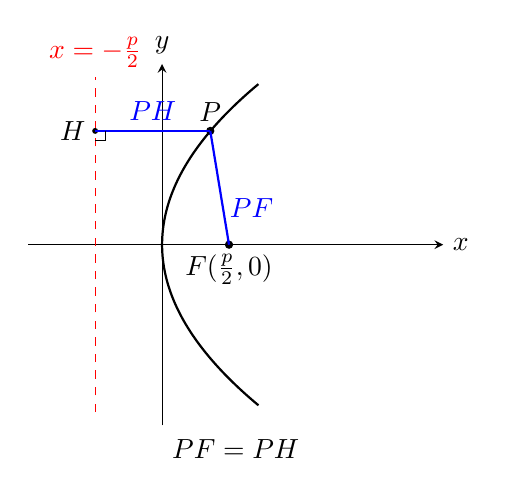
\begin{tikzpicture}[scale=0.85,>=stealth]
			\def\p{2}
			\pgfmathsetmacro{\f}{\p/2}
			\pgfmathsetmacro{\px}{0.72}
			\pgfmathsetmacro{\py}{1.7}
			
			\draw[->] (-2,0)--(4.2,0) node[right]{$x$};
			\draw[->] (0,-2.7)--(0,2.7) node[above]{$y$};
			
			\draw[thick,domain=-2.4:2.4,samples=100,smooth]
			plot ({\x*\x/(2*\p)},\x);
			
			\draw[dashed,red] (-\f,-2.5)--(-\f,2.5) node[above]{$x=-\frac p2$};
			
			\coordinate (F) at (\f,0);
			\coordinate (P) at (\px,\py);
			\coordinate (H) at (-\f,\py);
			
			\draw[fill] (F) circle (1.5pt) node[below]{$F(\frac p2,0)$};
			\draw[fill] (P) circle (1.5pt) node[above]{$P$};
			\draw[fill] (H) circle (1pt) node[left]{$H$};
			
			\draw[blue,thick] (P)--(F) node[midway,below right]{$PF$};
			\draw[blue,thick] (P)--(H) node[midway,above]{$PH$};
			
			\draw ($(H)+(0.15,0)$)--($(H)+(0.15,-0.15)$)--($(H)+(0,-0.15)$);
			
			\node at (1.1,-3.05) {$PF=PH$};
		\end{tikzpicture}
	\end{center}
	
	
	\subsection{抛物线的焦点弦}
	
	对于抛物线
	\[
	y^2=2px,
	\]
	过焦点 $F$ 的弦 $AB$ 称为焦点弦。若焦点弦与 $x$ 轴夹角为 $\theta$，则
	\[
	AB=\frac{2p}{\sin^2\theta}.
	\]
	
	\begin{center}
		\begin{tikzpicture}[scale=0.85,>=stealth]
			\def\p{2}
			\pgfmathsetmacro{\f}{\p/2}
			
			\draw[->] (-2,0)--(4.5,0) node[right]{$x$};
			\draw[->] (0,-3)--(0,3) node[above]{$y$};
			
			\draw[thick,domain=-2.6:2.6,samples=100,smooth]
			plot ({\x*\x/(2*\p)},\x);
			
			\coordinate (F) at (\f,0);
			\coordinate (A) at (0.45,1.35);
			\coordinate (B) at (2.7,-3.0);
			\coordinate (X) at (3.2,0);
			
			\draw[fill] (F) circle (1.5pt) node[below]{$F$};
			\draw[fill] (A) circle (1.5pt) node[above]{$A$};
			\draw[fill] (B) circle (1.5pt) node[right]{$B$};
			
			\draw[red,thick] (A)--(B);
			\draw[dashed] (F)--(X);
			
			\pic [draw, "$\theta$", angle radius=0.55cm, angle eccentricity=1.25]
			{angle=X--F--A};
			
			\node at (1.3,-3.45) {$AB=\dfrac{2p}{\sin^2\theta}$};
		\end{tikzpicture}
	\end{center}
	
	
	\subsection{抛物线的切线}
	
	对于
	\[
	y^2=2px,
	\]
	若切点为 $P(x_0,y_0)$，则切线方程为
	\[
	yy_0=p(x+x_0).
	\]
	
	\begin{center}
		\begin{tikzpicture}[scale=0.9,>=stealth]
			\def\p{2}
			\pgfmathsetmacro{\xzero}{0.8}
			\pgfmathsetmacro{\yzero}{sqrt(2*\p*\xzero)}
			
			\draw[->] (-1.5,0)--(4.2,0) node[right]{$x$};
			\draw[->] (0,-2.7)--(0,2.7) node[above]{$y$};
			
			\draw[thick,domain=-2.3:2.3,samples=100,smooth]
			plot ({\x*\x/(2*\p)},\x);
			
			\coordinate (P) at (\xzero,\yzero);
			\draw[fill] (P) circle (1.5pt) node[above]{$P(x_0,y_0)$};
			
			% 切线： y*y0 = p(x+x0)，即 y = p/y0 (x+x0)
			\draw[red,thick,domain=-1.2:3.3]
			plot (\x,{(\p/\yzero)*(\x+\xzero)}) node[right]{切线};
			
			\node at (1.1,-3.05) {$yy_0=p(x+x_0)$};
		\end{tikzpicture}
	\end{center}
	
	
	\subsection{点差法图形}
	
	点差法常用于处理中点弦问题。其基本结构是：设直线与圆锥曲线交于
	\[
	A(x_1,y_1),\qquad B(x_2,y_2),
	\]
	中点为
	\[
	M(x_0,y_0).
	\]
	
	\begin{center}
		\begin{tikzpicture}[scale=0.9,>=stealth]
			\def\a{3}
			\def\b{1.5}
			
			\draw[->] (-3.7,0)--(3.8,0) node[right]{$x$};
			\draw[->] (0,-2.0)--(0,2.1) node[above]{$y$};
			\draw[thick] (0,0) ellipse (\a cm and \b cm);
			
			\coordinate (A) at (-1.8,-1.2);
			\coordinate (B) at (2.0,1.15);
			\coordinate (M) at ($(A)!0.5!(B)$);
			
			\draw[red,thick] (A)--(B);
			\draw[blue,dashed] (0,0)--(M);
			
			\draw[fill] (A) circle (1.5pt) node[below left]{$A(x_1,y_1)$};
			\draw[fill] (B) circle (1.5pt) node[above right]{$B(x_2,y_2)$};
			\draw[fill] (M) circle (1.5pt) node[above left]{$M(x_0,y_0)$};
			
			\node at (0,-2.55) {点差法：由两点方程相减得到弦斜率};
		\end{tikzpicture}
	\end{center}
	
	对于椭圆
	\[
	\frac{x^2}{a^2}+\frac{y^2}{b^2}=1,
	\]
	若弦 $AB$ 的中点为 $M(x_0,y_0)$，则
	\[
	k_{AB}=-\frac{b^2x_0}{a^2y_0}.
	\]
	又因为
	\[
	k_{OM}=\frac{y_0}{x_0},
	\]
	所以
	\[
	k_{AB}k_{OM}=-\frac{b^2}{a^2}.
	\]
	
	对于双曲线
	\[
	\frac{x^2}{a^2}-\frac{y^2}{b^2}=1,
	\]
	有
	\[
	k_{AB}=\frac{b^2x_0}{a^2y_0},
	\]
	因此
	\[
	k_{AB}k_{OM}=\frac{b^2}{a^2}.
	\]
	
	对于抛物线
	\[
	y^2=2px,
	\]
	若弦 $AB$ 的中点为 $M(x_0,y_0)$，则
	\[
	k_{AB}=\frac{p}{y_0}.
	\]
	
	
	\subsection{三线模型}
	
	课件中多次出现的“三线模型”可以概括为：焦点、动点、切线或弦构成的角度关系。
	这类问题常用余弦定理、正弦定理、面积公式和离心率公式处理。
	
	\begin{center}
		\begin{tikzpicture}[scale=0.95,>=stealth]
			\coordinate (F1) at (-2.7,0);
			\coordinate (F2) at (2.7,0);
			\coordinate (P) at (0.8,1.8);
			\coordinate (A) at (-0.8,-0.6);
			\coordinate (B) at (2.4,0.9);
			
			\draw[->] (-3.4,0)--(3.6,0) node[right]{$x$};
			\draw[->] (0,-1.2)--(0,2.5) node[above]{$y$};
			
			\draw[fill] (F1) circle (1.5pt) node[below]{$F_1$};
			\draw[fill] (F2) circle (1.5pt) node[below]{$F_2$};
			\draw[fill] (P) circle (1.5pt) node[above]{$P$};
			
			\draw[blue,thick] (F1)--(P)--(F2);
			\draw[red,thick] (A)--(B) node[right]{$l$};
			
			\pic [draw, "$\alpha$", angle radius=0.45cm, angle eccentricity=1.3]
			{angle=F1--P--B};
			\pic [draw, "$\beta$", angle radius=0.65cm, angle eccentricity=1.3]
			{angle=B--P--F2};
			
			\node at (0,-1.65) {三线模型：焦点线、动点线、切线或弦};
		\end{tikzpicture}
	\end{center}
	
	
	\section{原教案图形链的补充还原}

	\subsection{六种定义中的第三、第四、第五与第六定义}

	\paragraph{第三定义：定点斜率乘积模型（点差法的几何原型）}
	设 $A(-a,0),B(a,0)$。若 $P(x_0,y_0)$ 在椭圆
	$\dfrac{x^2}{a^2}+\dfrac{y^2}{b^2}=1$ 上，则
	\[
	 k_{PA}k_{PB}
	 =\frac{y_0}{x_0+a}\cdot\frac{y_0}{x_0-a}
	 =\frac{y_0^2}{x_0^2-a^2}=-\frac{b^2}{a^2}.
	\]
	若 $P$ 在双曲线 $\dfrac{x^2}{a^2}-\dfrac{y^2}{b^2}=1$ 上，则
	\[
	 k_{PA}k_{PB}=\frac{b^2}{a^2}=e^2-1.
	\]
	当标准方程的焦点在 $y$ 轴上时，只需交换 $x,y$ 的角色。这正是课堂中
	“点差法”能够迅速得到弦斜率与中点坐标关系的图形依据。

	\begin{center}
	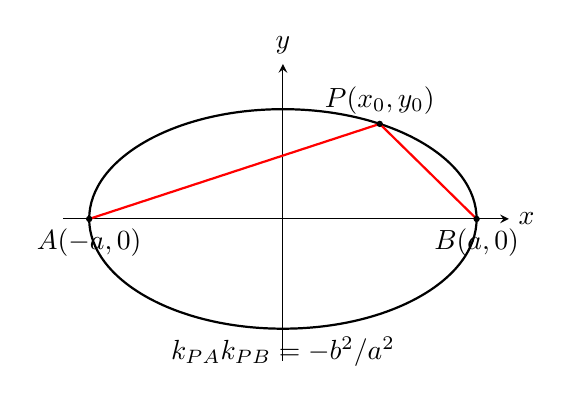
\begin{tikzpicture}[scale=.82,>=stealth]
	  \draw[->](-3.4,0)--(3.5,0)node[right]{$x$};
	  \draw[->](0,-2.2)--(0,2.4)node[above]{$y$};
	  \draw[thick] (0,0) ellipse (3 and 1.7);
	  \coordinate (A) at (-3,0); \coordinate (B) at (3,0);
	  \coordinate (P) at (1.5,1.472);
	  \draw[red,thick](A)--(P)--(B);
	  \fill (A)circle(1.4pt)node[below]{$A(-a,0)$};
	  \fill (B)circle(1.4pt)node[below]{$B(a,0)$};
	  \fill (P)circle(1.4pt)node[above]{$P(x_0,y_0)$};
	  \node at (0,-2.05) {$k_{PA}k_{PB}=-b^2/a^2$};
	\end{tikzpicture}
	\end{center}

	\paragraph{第四定义：同心圆投影构造}
	取同心圆 $O(a)$ 与 $O(b)$。同一条过 $O$ 的射线分别交两圆于 $M,N$，
	过 $M$ 作竖线、过 $N$ 作横线，两线交于 $P$，则
	$P=(a\cos\theta,b\sin\theta)$，故
	\[
	 \frac{x_P^2}{a^2}+\frac{y_P^2}{b^2}=1.
	\]
	若将两个投影改为和差组合，则得到双曲线的参数表示
	$(a\sec\theta,b\tan\theta)$。这一构造把“圆的匀速参数”转化为圆锥曲线。

	\paragraph{第五、六定义：丹德林球与圆锥截线}
	在圆锥内放置与截面及圆锥侧面均相切的球，球与截面的切点就是焦点。
	由同一点引球的切线段相等，可直接得到
	\[
	 PF_1+PF_2=2a\quad\text{或}\quad |PF_1-PF_2|=2a.
	\]
	若圆锥母线与轴的夹角为 $\alpha$，截面与轴的夹角为 $\beta$，则
	\[
	 e=\frac{\cos\beta}{\cos\alpha}.
	\]
	于是 $\beta>\alpha,\beta=\alpha,\beta<\alpha$ 分别对应椭圆、抛物线、双曲线。

	\subsection{焦点三角形的完整结论链}

	设 $P$ 为椭圆上一点，$\theta=\angle F_1PF_2$。令
	$m=PF_1,n=PF_2$，则
	\[
	 m+n=2a,\qquad F_1F_2=2c,qquad
	 mn=\frac{2b^2}{1+\cos\theta}.
	\]
	因此
	\[
	 S_{\triangle PF_1F_2}
	 =\frac12mn\sin\theta=b^2\tan\frac\theta2.
	\]
	当 $P$ 位于短轴端点时，$\theta$ 最大；焦半径均落在区间
	$[a-c,a+c]$ 内。若已知 $mn=\lambda$，则
	\[
	 S_{\triangle PF_1F_2}=b\sqrt{\lambda-b^2}.
	\]
	若 $OP=\lambda$，由中线公式
	$OP^2=\tfrac12(PF_1^2+PF_2^2)-c^2$ 可得
	\[
	 PF_1PF_2=2a^2-c^2-\lambda^2,qquad
	 S_{\triangle PF_1F_2}=b\sqrt{a^2-\lambda^2}.
	\]

	对双曲线右支上的点 $P$，令
	$\theta=\angle F_1PF_2$，则 $PF_1-PF_2=2a$，并有
	\[
	 PF_1PF_2=\frac{2b^2}{1-\cos\theta},qquad
	 S_{\triangle PF_1F_2}=b^2\cot\frac\theta2.
	\]
	若 $PF_1PF_2=\lambda$，则同样可以写成
	\[
	 S_{\triangle PF_1F_2}=b\sqrt{\lambda-b^2}.
	\]
	这说明椭圆与双曲线在“焦半径乘积已知”时具有同一面积表达式，
	差别只在乘积与夹角的换算式。

	\paragraph{三焦点模型}
	若同一点 $P$ 同时属于焦轴重合的一条椭圆和一条双曲线，且两曲线离心率
	分别为 $e_1,e_2$，课堂图形中的两个焦点角可化为同一个角 $\theta$，从而得到
	\[
	 \boxed{\frac{\sin^2\theta}{e_1^2}+\frac{\cos^2\theta}{e_2^2}=1}.
	\]
	它把椭圆的“和”与双曲线的“差”统一到一个三角恒等式中。

	\subsection{焦点弦、比例与离心率}

	椭圆中，设过右焦点 $F$ 的弦 $AB$ 与正向 $x$ 轴夹角为 $\theta$，
	半通径 $p=b^2/a$，则
	\[
	 AF=\frac{p}{1-e\cos\theta},\qquad
	 BF=\frac{p}{1+e\cos\theta},
	\]
	\[
	 AB=\frac{2p}{1-e^2\cos^2\theta},qquad
	 \frac1{AF}+\frac1{BF}=\frac2p.
	\]
	若 $AF=\lambda BF$，则
	\[
	 \boxed{e\cos\theta=\left|\frac{\lambda-1}{\lambda+1}\right|}.
	\]
	该式是原稿中多道“给出线段倍数求离心率”图形题的共同核心。

	双曲线中应先判断弦端点所在支。若两点位于同一支，焦半径取
	$|ex-a|$；若穿过两支，必须使用有向距离或分支讨论，不能直接照搬椭圆公式。
	在右支且焦点弦不跨支的常用情形，仍可由
	$PF_1=ex+a,PF_2=ex-a$ 与比例条件求 $e$。

	\subsection{双曲线渐近线与特征三角形}

	双曲线
	\[
	 \frac{x^2}{a^2}-\frac{y^2}{b^2}=1
	\]
	的渐近线为 $y=\pm\dfrac ba x$。记右焦点 $F(c,0)$，则
	\[
	 T\left(\frac{a^2}{c},\frac{ab}{c}\right)
	\]
	同时满足 $OT=a$、$TF=b$、$OT\perp TF$。这个直角三角形就是原稿反复使用的
	“特征三角形”，三边恰为 $a,b,c$。

	若 $P(x_0,y_0)$ 在双曲线上，$d_1,d_2$ 为 $P$ 到两条渐近线的距离，则
	\[
	 d_1d_2
	 =\frac{|bx_0-ay_0|\,|bx_0+ay_0|}{a^2+b^2}
	 =\boxed{\frac{a^2b^2}{c^2}}.
	\]
	所以双曲线上任一点到两条渐近线距离之积为定值。

	\begin{center}
	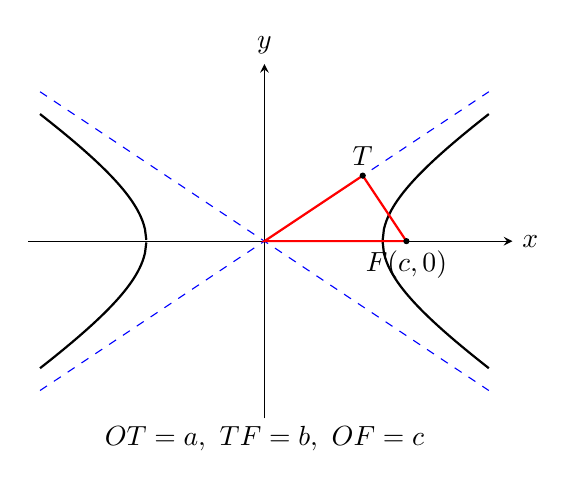
\begin{tikzpicture}[scale=.75,>=stealth]
	 \draw[->](-4,0)--(4.2,0)node[right]{$x$};
	 \draw[->](0,-3)--(0,3)node[above]{$y$};
	 \draw[dashed,blue](-3.8,-2.53)--(3.8,2.53);
	 \draw[dashed,blue](-3.8,2.53)--(3.8,-2.53);
	 \draw[thick,domain=2:3.8,samples=80]plot(\x,{.666*sqrt(\x*\x-4)});
	 \draw[thick,domain=2:3.8,samples=80]plot(\x,{-.666*sqrt(\x*\x-4)});
	 \draw[thick,domain=-3.8:-2,samples=80]plot(\x,{.666*sqrt(\x*\x-4)});
	 \draw[thick,domain=-3.8:-2,samples=80]plot(\x,{-.666*sqrt(\x*\x-4)});
	 \coordinate(O)at(0,0);\coordinate(F)at(2.404,0);\coordinate(T)at(1.664,1.109);
	 \draw[red,thick](O)--(T)--(F)--cycle;
	 \fill(F)circle(1.5pt)node[below]{$F(c,0)$};
	 \fill(T)circle(1.5pt)node[above]{$T$};
	 \node at(0,-3.35){$OT=a,\ TF=b,\ OF=c$};
	\end{tikzpicture}
	\end{center}

	\section{抛物线图形性质的系统还原}

	以下统一设抛物线 $C:y^2=2px\ (p>0)$，焦点
	$F(\tfrac p2,0)$，准线 $l:x=-\tfrac p2$。

	\subsection{焦点弦的代数骨架}
	设过焦点的弦 $AB$ 端点为 $A(x_1,y_1),B(x_2,y_2)$，则
	\[
	 x_1x_2=\frac{p^2}{4},\qquad y_1y_2=-p^2,qquad
	 \overrightarrow{OA}\cdot\overrightarrow{OB}=-\frac34p^2,
	\]
	\[
	 k_{OA}k_{OB}=-4,qquad
	 k_{AB}=\frac{2p}{y_1+y_2}.
	\]
	弦 $AB$ 的方程可写成
	\[
	 \boxed{(y_1+y_2)y=2px+y_1y_2}.
	\]
	更一般地，若弦过轴上点 $(m,0)$，则 $x_1x_2=m^2$。

	若焦点弦与 $x$ 轴的夹角为 $\theta$，则
	\[
	 AF=\frac{p}{1-\cos\theta},\qquad
	 BF=\frac{p}{1+\cos\theta},
	\]
	\[
	 AB=\frac{2p}{\sin^2\theta},qquad
	 \frac1{AF}+\frac1{BF}=\frac2p.
	\]
	并且
	\[
	 S_{\triangle AOB}=\frac{p^2}{2\sin\theta}.
	\]

	\subsection{切线、切点弦与定点}
	抛物线在 $A(x_1,y_1)$ 处的切线为
	\[
	 \boxed{yy_1=p(x+x_1)}.
	\]
	从点 $P(x_0,y_0)$ 引两条切线，切点为 $A,B$，则切点弦为
	\[
	 \boxed{y_0y=p(x+x_0)}.
	\]
	由此得到课堂中的三个定点结论：
	\begin{enumerate}
	 \item 若 $P$ 在准线上，则切点弦 $AB$ 恒过 $(\tfrac p2,0)$；
	 \item 若 $OA\perp OB$，则弦 $AB$ 恒过 $(2p,0)$；
	 \item 若弦 $AB$ 过轴上点 $(m,0)$，则两端切线交点在定直线
	 $x=-m$ 上；特别地，焦点弦两端切线的交点在准线上。
	\end{enumerate}

	\subsection{焦点弦的圆与直角性质}
	设 $A,B$ 为焦点弦端点，$M,N$ 分别是 $A,B$ 在准线上的投影，则：
	\begin{enumerate}
	 \item 以 $AB$ 为直径的圆与准线相切；
	 \item 以 $AF,BF$ 为直径的两圆均与 $y$ 轴相切；
	 \item $M,O,B$ 三点共线，$N,O,A$ 三点共线；
	 \item $MF\perp NF$；若两条切线交准线于 $Q$，则 $AQ\perp BQ$；
	 \item 过焦点作两条互相垂直的焦点弦 $AB,DE$，则
	 \[
	 \boxed{\frac1{AB}+\frac1{DE}=\frac1{2p}}.
	 \]
	\end{enumerate}

	\subsection{抛物线的光学性质}
	设 $M(x_0,y_0)$ 为抛物线上一点。切线斜率为 $p/y_0$，法线斜率为
	$-y_0/p$。法线与轴交于 $N(x_0+p,0)$，于是
	\[
	 NF=x_0+\frac p2=MF.
	\]
	所以 $\triangle MFN$ 为等腰三角形，切线平分焦半径 $MF$ 与过 $M$
	且平行于轴的射线所成的外角。这就是“从焦点发出的光线经抛物线反射后平行于轴”
	的解析证明。

	\subsection{椭圆与双曲线的光学性质（与原稿末页对应）}
	椭圆 $\dfrac{x^2}{a^2}+\dfrac{y^2}{b^2}=1$ 在
	$M(x_0,y_0)$ 处的切线为
	\[
	 \frac{xx_0}{a^2}+\frac{yy_0}{b^2}=1.
	\]
	法线斜率为 $\dfrac{a^2y_0}{b^2x_0}$。利用
	$MF_1=a+ex_0,MF_2=a-ex_0$ 可验证：法线平分
	$\angle F_1MF_2$，故从一个焦点发出的光线经椭圆反射后通过另一个焦点。
	双曲线同理，切线平分一条焦半径与另一条焦半径反向延长线所成的角，
	反射线看起来像从另一焦点发出。

	\subsection{圆锥曲线光学性质总结图}
	
	\begin{center}
		\begin{tikzpicture}[scale=0.75,>=stealth]
			
			% 椭圆
			\begin{scope}[xshift=0cm]
				\draw[thick] (0,0) ellipse (2.3 and 1.2);
				\coordinate (F1) at (-1.6,0);
				\coordinate (F2) at (1.6,0);
				\coordinate (P) at (0.4,1.15);
				
				\draw[fill] (F1) circle (1.3pt) node[below]{$F_1$};
				\draw[fill] (F2) circle (1.3pt) node[below]{$F_2$};
				\draw[fill] (P) circle (1.3pt) node[above]{$P$};
				
				\draw[blue,thick,->] (F1)--(P);
				\draw[blue,thick,->] (P)--(F2);
				\draw[red,thick] (-1.1,1.6)--(1.8,0.65);
				
				\node at (0,-1.65) {椭圆};
				\node at (0,-2.1) {$F_1\to P\to F_2$};
			\end{scope}
			
			% 双曲线
			\begin{scope}[xshift=5.4cm]
				\draw[thick,domain=1.0:2.8,samples=80,smooth]
				plot (\x,{0.7*sqrt(\x*\x-1)});
				\draw[thick,domain=1.0:2.8,samples=80,smooth]
				plot (\x,{-0.7*sqrt(\x*\x-1)});
				
				\coordinate (F1) at (-1.6,0);
				\coordinate (F2) at (1.6,0);
				\coordinate (P) at (2.2,1.2);
				
				\draw[fill] (F1) circle (1.3pt) node[below]{$F_1$};
				\draw[fill] (F2) circle (1.3pt) node[below]{$F_2$};
				\draw[fill] (P) circle (1.3pt) node[above]{$P$};
				
				\draw[blue,thick] (P)--(F1);
				\draw[blue,thick] (P)--(F2);
				\draw[red,thick] (1.2,1.75)--(2.9,0.45);
				
				\node at (1.0,-1.65) {双曲线};
				\node at (1.0,-2.1) {切线平分焦半径夹角};
			\end{scope}
			
			% 抛物线
			\begin{scope}[xshift=10.5cm]
				\def\p{1.6}
				\draw[thick,domain=-1.8:1.8,samples=80,smooth]
				plot ({\x*\x/(2*\p)},\x);
				
				\coordinate (F) at (0.8,0);
				\coordinate (P) at (0.7,1.5);
				
				\draw[fill] (F) circle (1.3pt) node[below]{$F$};
				\draw[fill] (P) circle (1.3pt) node[above]{$P$};
				
				\draw[blue,thick,->] (F)--(P);
				\draw[blue,thick,->] (P)--(2.7,1.5);
				\draw[red,thick] (-0.3,1.95)--(1.8,0.75);
				
				\node at (1.0,-1.65) {抛物线};
				\node at (1.0,-2.1) {反射后平行于轴};
			\end{scope}
			
		\end{tikzpicture}
	\end{center}
	
\end{document}
